\section{Sentiment over time} 

Collection of a large sample of users and their tweets in practice is
longitudinal in time. Practical bandwidth limits (but in our
case API rate limits) constrain the number of users collected per day.
The probability of sentiments can greatly change conditioned on the
day because of events (like holidays) and periodic behavior (like days
of the week). For this reason, we examine Twitter sentiment across
time. 

Figure~\ref{fig:time} shows the distribution of tweet
creation time for the tweets in our labeled dataset. Tweets were
labeled 23.9\% positive and 14.3\% negative. Recall that the
tweet we used for a collected user was their latest tweet (``status'')
at the time of collection. Therefore the distribution of tweets over
time is a result of \emph{both} the rate of collection at each time
(controlled by us) and the rate of tweet creation at the time (not
controlled). The boost toward the end of the month is partly
explained by a more aggressive collection of 3 parallel random walks
at once using the 3 Twitter accounts of the authors, and partly
explained by the holiday. The rate tapers off as we finished up our
collection the chains and the holiday ends. The dip in the
middle of the high-rate collection period is partly due to some time
when we baby-sat collection less closely; collection can fail and
require restarts in the case of unforeseen Twitter server errors.

\begin{figure}[htb]
\begin{center}
  \includegraphics[width=0.9\columnwidth]{figs/time.png}
\begin{minipage}{0.9\columnwidth}
\end{minipage}
\end{center}
\caption{Tweet creation date for tweets collected during November 2012, for the \emph{labeled
        subset} of 2800 English tweets.}
\label{fig:time}
\end{figure}


Figure~\ref{fig:november} and~\ref{fig:november2} show the proportion of positve-labeled
tweets over the collection period. Holidays tend to be more positive.
More positive tweets were posted after Election Day. Weekends tend to
be more positive than the end of the week and have more neutral
tweets due to higher activity. Black Friday was the only day to have
more negative tweets than positive.

\begin{figure*}[htb]
    \minipage{0.5\linewidth}
      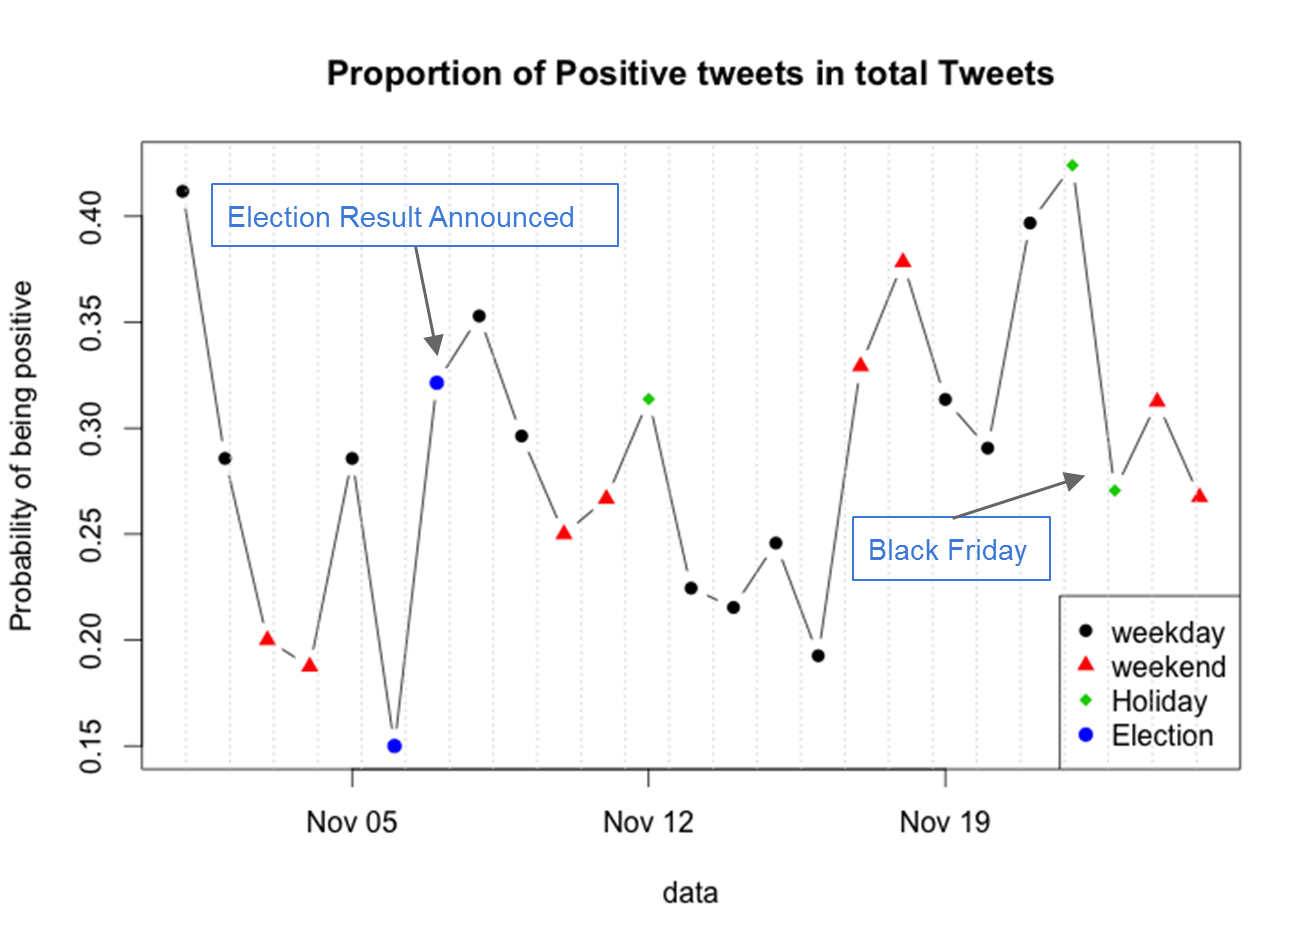
\includegraphics[width=\linewidth]{figs/sentiment.png}
\caption{Probability of postive tweets for each day of the collection period in November 2012.}
\label{fig:november}
    \endminipage\hfill
    \minipage{0.5\linewidth}
      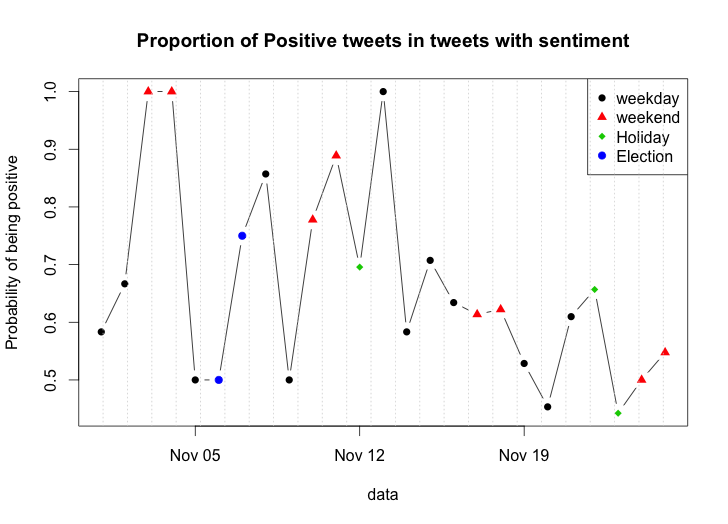
\includegraphics[width=\linewidth]{figs/sentiment2.png}
\caption{Probability of postive tweets out of sentimental tweets.}
\label{fig:november2}
    \endminipage
\end{figure*}

%%%\begin{figure}[htb]
%%%\begin{center}
%%%  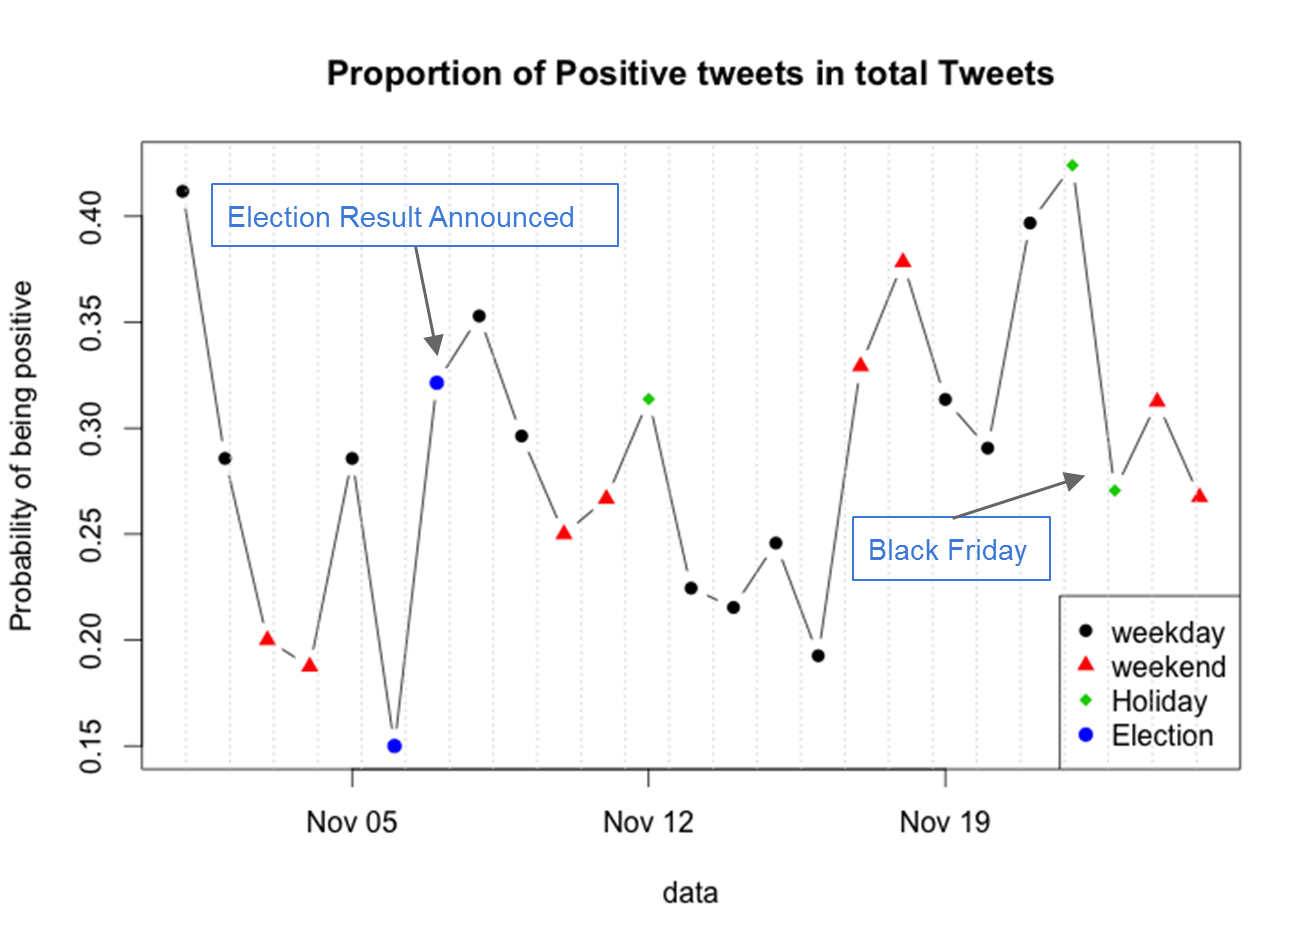
\includegraphics[width=0.9\columnwidth]{figs/sentiment.png}
%%%\begin{minipage}{0.9\columnwidth}
%%%\end{minipage}
%%%\end{center}
%%%\caption{Probability of postive tweetsover the collection period in November 2012.}
%%%\label{fig:november}
%%%\end{figure}


